%%=====================================================================================
%%
%%       Filename:  Assignment6.tex
%%
%%    Description:  Solution to assignment 6.
%%
%%        Version:  1.0
%%        Created:  03/28/2017
%%       Revision:  none
%%
%%         Author:  Dilawar Singh (), dilawars@ncbs.res.in
%%   Organization:  NCBS Bangalore
%%      Copyright:  Copyright (c) 2017, Dilawar Singh
%%
%%          Notes:  
%%                
%%=====================================================================================

\documentclass[a4paper,10pt]{article}
\usepackage[margin=20mm]{geometry}
\usepackage{pgf,tikz}
\usepackage{amsmath}
\usepackage{amssymb}
\usepackage{verbatim}
\usepackage{hyperref}
\usepackage{pgfplots}

\usetikzlibrary{shapes,backgrounds,decorations,decorations.pathmorphing}
% Title Page
\title{Solution : Homework 6} 
\author{Dilawar Singh}
\date{\today}
\begin{document}
\maketitle

The simulation is done in Haskell;  Since Haskell is not a very mainstream
language, code is in appendix for your reference only. It is available on
demand. It can also be downloaded 
\href{https://raw.githubusercontent.com/dilawar/Courses/master/TASHIP/StochasticProcess2017/Assignment6/solution.hs}{from
github}.

\section{Solution}

For each case we plot 5 sample trajectories.

\foreach \vel in {0,10}
{
    \foreach \dt in {0.1, 0.01, 0.001}
    {
        \pgfmathsetmacro\everyN{round(1.0/\dt)}
        \begin{tikzpicture}[scale=1]
            \begin{axis}[
                    xlabel=Time (au) ,ylabel= Position (au)
                    , grid style={draw=gray!20}
                    , grid = both
                    , title =  $v_0$ \vel\; and dt \dt
                    , width = 3cm, scale only axis
                    , no marks
                    ]
                \foreach \i in {1,2,3,4,5}
                {
                    \addplot  gnuplot [ raw gnuplot ] {
                        set datafile separator ",";
                        plot "./_data/\vel _\dt _\i .txt" using 1:3 every \everyN with lines;
                    };
                }
            \end{axis}
        \end{tikzpicture}
    }
    \par
}

Next, we plot the histogram if velocity.

\foreach \vel in {0,10}
{
     Collect all data in one file. Last entry from each file.
    \foreach \dt in {0.1, 0.01, 0.001}
    {
        \pgfmathsetmacro\everyN{round(1.0/\dt)}
        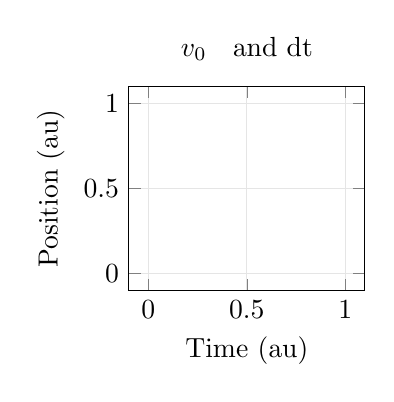
\begin{tikzpicture}[scale=1]
            \begin{axis}[
                    xlabel=Time (au) ,ylabel= Position (au)
                    , grid style={draw=gray!20}
                    , grid = both
                    , title =  $v_0$ \vel\; and dt \dt
                    , width = 3cm, scale only axis
                    , no marks
                    ]
                \foreach \i in {1,2,...,100}
                {
                    %\addplot  gnuplot [ raw gnuplot ] {
                        %set datafile separator ",";
                        %plot "./_data/\vel _\dt _\i .txt" using 1:3 every \everyN with lines;
                    %};
                }
            \end{axis}
        \end{tikzpicture}
    }
    \par
}


\newpage
\appendix
\section{Haskell based simulator}
\verbatiminput{./solution.hs}

\end{document}          
